\documentclass[border=15pt, multi, tikz]{standalone}
\usepackage{import}
\usepackage{ctex}% 中文支持
\usepackage{tikz}

\subimport{./}{init}
\usetikzlibrary{positioning}
\usetikzlibrary{3d} %for including external image
\usetikzlibrary{quotes,angles}
\usetikzlibrary{calc}
\usetikzlibrary{decorations.pathreplacing}

\def\DataColor{rgb:blue,5;white,5}
\def\ConvColor{rgb:yellow,5;red,2.5;white,5}
\def\ConvReluColor{rgb:yellow,5;red,5;white,5}
\def\PoolColor{rgb:red,1;black,0.3}
\def\PcColor{rgb:blue,5;red,2.5;white,5}
\def\PcSquashColor{rgb:blue,5;red,5;white,4}
\def\DcColor{rgb:blue,5;green,15}
\def\SumColor{rgb:blue,5;green,15}
% \def\SoftmaxColor{rgb:magenta,5;black,7}

\begin{document}
\begin{tikzpicture}

\tikzstyle{connection}=[ultra thick,every node/.style={sloped,allow upside down},draw=\edgecolor,opacity=0.7]

\node[] at (-6, 0, 0) {机器人在环境中探索到的数据};
%%%%%%%%%%%%%%%%%%%%%%%%%%%%%%%%%%%%%%%%%%%%%%%%%%%%%%%%%%%%%%%%%%%%%%%%%%%%%%%%%%%%%%%%
%% buffer
%%%%%%%%%%%%%%%%%%%%%%%%%%%%%%%%%%%%%%%%%%%%%%%%%%%%%%%%%%%%%%%%%%%%%%%%%%%%%%%%%%%%%%%%
% 缓冲buffer
\pic[shift={(0, 0, 0)}] at (0, 0, 0) {Box={name=buffer1,fill=\PoolColor,opacity=0.5,height=24,width=2,depth=24}};
% out_buffer
\pic[shift={(20, 0, 0)}] at (buffer1-east) {Box={name=out_buffer,fill=\PoolColor,opacity=0.5,height=30,width=14,depth=30}};
% positive_buffer
\pic[shift={(10, 0, 15)}] at (buffer1-east) {Box={name=positive_buffer,fill=\PoolColor,opacity=0.5,height=30,width=7,depth=30}};


% 注释
\node[] at (0, -4, 0) {缓冲buffer};
\node[] at (21, -5, 0) {输出buffer};
\node[] at (10, -5, 15) {正激励buffer};
\node[] at (5, -1, 15) {写入成功数据};
\node[] at (10, 1, 0) {写入数据};
\node[] at (19, -1, 15) {每隔一段时间检查输出buffer是否有足够多的成功数据,写入成功数据};
% 卷积单元之间的连接
\draw [connection]  (buffer1-east) -- node {\midarrow}(out_buffer-west);
% 卷积单元的注释
% 数据输入
\draw[connection] (-3, 0, 0) -- node {\midarrow} (buffer1-west);
\path (buffer1-east) -- (out_buffer-west) coordinate[pos=0.4] (after1);
\draw[connection] (1, 0, 4) -- node {\midarrow}(1, 0, 15) -- node {\midarrow} (positive_buffer-west);
\draw[connection] (positive_buffer-east) -- node {\midarrow}(22, 0, 15) -- node {\midarrow} (22, 0, 5);
%%%%%%%%%%%%%%%%%%%%%%%%%%%%%%%%%%%%%%%%%%%%%%%%%%%%%%%%%%%%%%%%%%%%%%%%%%%%%%%%%%%%%%%%
%% Data
%%%%%%%%%%%%%%%%%%%%%%%%%%%%%%%%%%%%%%%%%%%%%%%%%%%%%%%%%%%%%%%%%%%%%%%%%%%%%%%%%%%%%%%%
\node[canvas is zy plane at x=0] (temp) at (30,0,0) {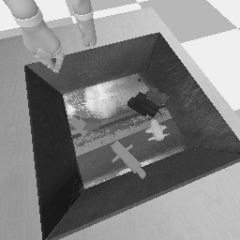
\includegraphics[width=6cm,height=6cm]{observation.png}};
\draw[connection] (out_buffer-east) -- node {\midarrow} (28, 0, 0);


\end{tikzpicture}
\end{document}
